\chapter{The Radio Interferometric Measurement Equation}
In this chapter we give the reader a ``grand tour'' \footnote{It is important to stress that radio astronomy is a cross-section of many disciplines including astronomy, physics, 
electrical engineering and, increasingly, high performance and distributed computing. The following texts provide further insight for those with a computing background (we recommend 
reading the first three texts in order before moving to synthesis imaging):
\begin{itemize}
 \item \textit{Antennas: Fundamentals, Design, Measurement} \cite{blake2009antennas} serves as a good introductory text on general [communications] radio antenna design from an electrical engineering perspective. Chapters 1 through 4
 are very insightful.
 \item \textit{A Scientist and Engineer's guide to Digital Signals Processing} \cite{smith1997scientist}. Available freely at \url{http://www.dspguide.com/}. A must-read introduction to core digital 
 signals processing techniques, which cover sampling theory, introductory filter design and a good starter on the practical uses of Fourier transforms.
 \item \textit{Radio telescopes} \cite{christiansenradiotelescopes} gives insight into the historic development of radio telescopes from the 1930s through to the 1960s, with a focus on telescope design, interferometry, measurement and a 
 good overview of the field of radio astronomy from an engineering perspective. The book is in the public domain and freely available from \url{https://archive.org/details/Radiotelescopes}.
 \item \textit{Synthesis Imaging In Radio Astronomy II} \cite{taylor1999synthesis}. A very useful (and beginner-friendly) collection of lectures on synthesis imaging, covering the domain of radio astronomical imaging 
 in its entirety.
 \item \textit{Interferometry and Synthesis in Radio Astronomy} \cite{thompson2008interferometry} covers the imaging pipeline in great detail from correlation through calibration, cleaning
 and beyond. A very valuable reference.
\end{itemize}
} of how radio telescopes make measurements of the radio sky. A mathematical model relating the radio sky to these measurements is derived,
and in the chapter on synthesis imaging we'll discuss the inversion of this model and some of the complications that arise when doing so.
\section{The radio universe}
Just as with visible light, radio waves are a form of electromagnetic radiation (consisting of waves with an electrical and perpendicular magnetic component), which propagates through free space at the speed 
of light. Recall from elementary physics that the frequency and wavelength of a wave are related:
\begin{equation*}
 \nu = \frac{v}{\lambda}
\end{equation*}
where: $\nu$ is the frequency, $\lambda$ is the wavelength and $v$ is the velocity of the propagation of the wave in some propagation medium\\

In a vacuum and far away from obstacles (\textit{free space}) electromagnetic waves propagate at a constant velocity, $c\approx 3\text{x}10^8m.s^{-1}$. This velocity is only slightly reduced
when propagating though most other media. We can conveniently measure these wavefronts with telescopes of various form at either ground-level or from planetary orbit. 

Generally speaking, black bodies (sources that near-perfectly absorb all incoming electromagnetic radiation) will radiate this energy over a very wide 
band of the electromagnetic spectrum. See Figure~\ref{fig_plank}. 

\begin{figure}[ht]
 \begin{mdframed}
 \centering
 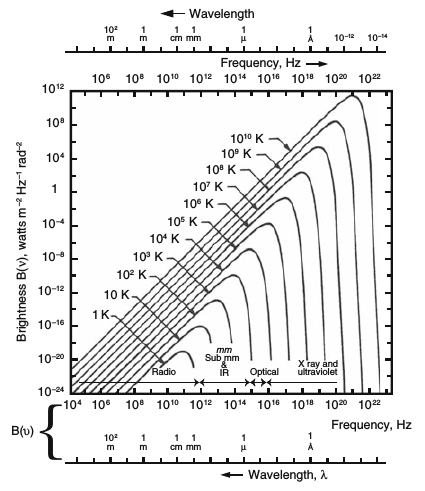
\includegraphics[width=0.4\textwidth]{images/plank_dist.png}
 \caption[Black body radiation]{The radiation intensity distribution for a black body in equilibrium. The intensity distribution of black-body emission depends on both the equilibrium temperature of the body and 
  the frequency of emission alluded to earlier. A black-body in equilibrium will, on average, have an emission intensity distribution that roughly follows the Plank 
  distribution. Taken from \textit{Tools of Radio Astronomy} \cite{wilson2009tools}}
  \label{fig_plank}
 \end{mdframed}
\end{figure}

Large bodies like planets and stars are generally considered to be of this type. Black bodies have to be very hot 
in order to be observed in radio if they are significantly far outside our solar system. One would expect the radio sky to be
quite empty if this was the only source of radio emission in nature and it placed a damper on radio observation until 
Karl Jansky's observation of radio electromagnetic radiation stemming from cosmic sources in the early 1930s sparked interest in observing 
this region of the spectrum. 

We know now that electromagnetic energy can be emitted by both thermal and non-thermal sources. These thermal sources not only include
black bodies, but can also include, for example, ionized gasses, such as ionized hydrogen. On the other hand, a good example of 
non-thermal emission is the synchrotron emission by electrons accelerated radially through magnetic fields. 
An example of a source of the latter are pulsars. 

One would expect radio waves to have the same optical properties as visible light, since they too are a form of electromagnetic radiation. These are, respectively, reflection, refraction (bending as these waves propagate
through mediums of different densities), diffraction and interference. The last two phenomena are of particular importance in our discussion on radio telescopes and can only be described using
physical optics. Interference can either be constructive or destructive by nature. When two or more waves collide the resulting wave will be the sum total of the colliding waves. If the incoming waves are perfectly 
in phase (their crests line up perfectly) the resulting wave will have the combined amplitude of the contributing waves. However, if they are out of phase the resulting wave may have significantly reduced amplitude. 
As for diffraction, Huygens' principle states that each point on an incoming wavefront (either planar or curved) acts as a point source on its own. The secondary waves produced by each of these point sources 
propagates forward radially and a new wavefront is formed where they experience maximum constructive interference. This explains why even planar waves can seemingly ``bend'' around obstacles.

In free space the total energy along the wavefront is conserved as it propagates forward, provided 
the wavefront is of reasonable extent (significantly longer than a wavelength). This also means that the energy density 
on each of these wavefronts will decay at a rate proportional to the square of the distance between the front and its emitting source, hence
the requirement that the emitting source is sufficiently far away from the observing telescope. 

When these waves propagate through some medium other than that of a vacuum the decrease in directional energy is not the only form of attenuation. In an
atmosphere, depending on the wavelength, some particles such as oxygen and water vapor will absorb and scatter a significant portion of the incoming 
energy (especially at shorter wavelengths). At the very long wavelengths the charged ionosphere is effectively opaque and acts as a good reflector. This may 
be ideal when trying to transmit signals very far beyond the horizon, but makes astronomical observation at such wavelengths impossible.  Due to these additional attenuation 
factors ground-based observation is effectively limited to the spectrum of visible light and the, vastly wider, radio band. Most of the in-between 
infrared spectrum is only observable at high altitudes and under dry conditions, see Figure~\ref{fig_radio_window}. 

In addition to the optical properties of electromagnetic waves and their attenuation one has to consider the direction of propagation of each point on the incoming wavefront. If most of the energy of these points is strongly 
directional the wave is said to be \textit{polarized}. For polarized emissions the path traced by each point (of either the electrical or magnetic components) will be highly regular; it will 
remain in a single plane (\textit{linear} polarization), will spiral at a fixed diameter (\text{circular} polarization) or will spiral elliptically. Circular polarized waves can be thought 
of as the combination of two perpendicular linearly polarized waves of equal strength (if the two wavefronts are not equally strong the resultant polarization will be elliptical). 

We can draw on an application of this property from an everyday context: in the visible spectrum sunglasses will filter out all light except vertically polarized light, in order to reduce glare. A single-feed radio 
antenna will similarly measure a single directional component, and will therefore only be useful in measuring strongly polarized sources. Such antennae are not useful for general observations, save for 
those of pulsars. In most contexts it is more useful to have two perpendicular feeds (a dipole is a simple example) in order to fully describe the incoming wavefront of the field parallel to the dipole (or at least 
the electric component thereof). When the energy measured by both feeds are roughly equal the emitting source is said to be \textit{unpolarized}.
\begin{figure}[ht]
 \begin{mdframed}
 \centering
 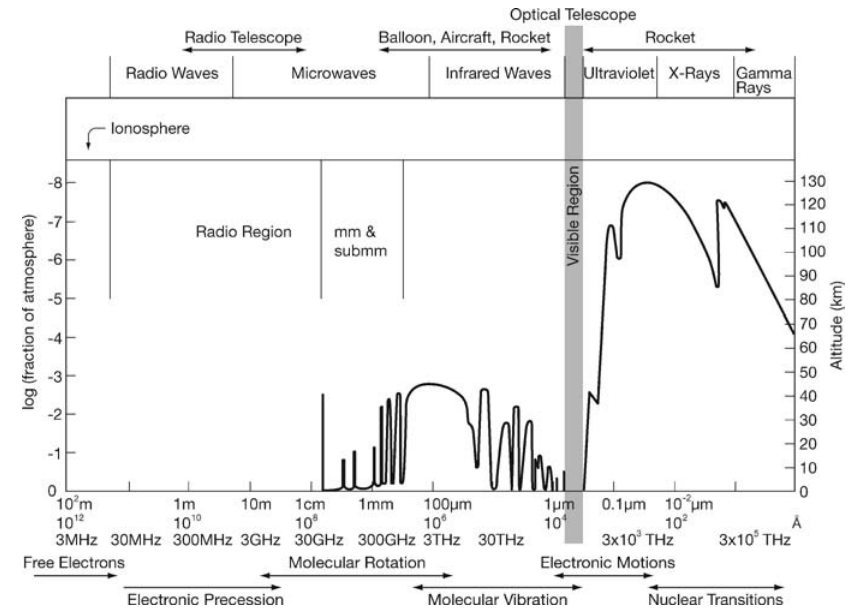
\includegraphics[width=0.6\textwidth]{images/radio_window.png}
 \caption[The radio window]{The radio window - Earth-based radio astronomy is bound to a range of wavelengths between $\lambda\approx 0.2mm$ and $\lambda\approx 20m$, by the molecular absorption bands of oxygen and water at
 shorter wavelengths and the ionosphere at longer wavelengths. The figure shows at what altitude the incoming electromagnetic radiation is attenuated by a factor of 0.5. Image taken from \textit{Tools of Radio Astronomy}~\cite{wilson2009tools}.}
 \label{fig_radio_window}
 \end{mdframed}
\end{figure}

Since the early days significant progress has been made towards increasing in the sensitivity and size of these radio telescopes. Next we will explore 
how a single-element telescope works, before moving onto the topic of aperture synthesis with array-based telescopes.

\section{Single antenna telescopes}
\subsection{Overview}
Maxwell's set of partial differential equations (1873) is one of the most elegant ways of explaining the relationship between electrical and magnetic fields, and how these can propagate at the speed of light 
though free space. In summary they state that a when current flows, a magnetic field is created in the surrounding space. When this magnetic field is varied an accompanying perpendicular electrical field is formed. This electrical field 
varies at the same frequency as the magnetic field, which in turn varies at the frequency at which the underlying current changes. Not only does this mean that antennae can generate electromagnetic fields and transmit signals, 
but in fact that any transmitting antenna can be used as a receiver and vice versa, assuming that it is capable of dealing with high voltages and is efficient enough for the particular application domain. Radio telescopes 
take the form of receivers and, as with terrestrial radio transmission, the extraterrestrial electromagnetic radiation will induce measurable current in the antenna - much more so at shorter wavelengths 
because of the opaqueness of the ionosphere at longer wavelengths.

To simplify our discussion we will only consider directional antennae (a simple parabolic reflector with an axial feed above the center of the parabola is 
one such choice). Here the parabolic reflector serves either to focus highly directional incoming energy to a single point, or conversely to 
focus the energy of the transmitter into a very narrow beam. Because the wavelengths of radio waves are the size of man-made objects the geometrical optics 
used in optical telescopes, where waves can be considered as rays, are of very limited use. It is much more preferable to describe these antennae in terms of 
physical optics.

Consider, for the moment, that the telescope is suspended in free space with no obstructions in its vicinity (including the ground or supports). If
we also (in blissful ignorance) discard the effects of the feed between this focus and measuring equipment, then the energy measured at the focus 
of the parabola should be the sum of contributions across the extent of the collected wavefront. However, instead of focusing all 
energy at one single point, as one would expect when using geometrical optics, an interference pattern is formed. Here
distinct beams are discernible (a close analogue to this is the interference pattern formed when light passes through a narrow slit).
If a cutting plane were to be placed horizontally at the focus of the parabola a single ``primary'' beam of maximum 
constructive interference would be noticed, along with several minor lobes to either side of that primary beam. The lobes right 
next to the primary beam are appropriately termed ``side'' lobes (refer to Figure\ref{diffraction_pattern}). A highly directional antenna 
limits the maximum amplitude of these lobes considerably. It is important to note that an isotropic antenna will not have a single primary 
lobe, but may have several main lobes of equal amplitude. 

\begin{figure}[ht]
 \begin{mdframed}
  \centering
  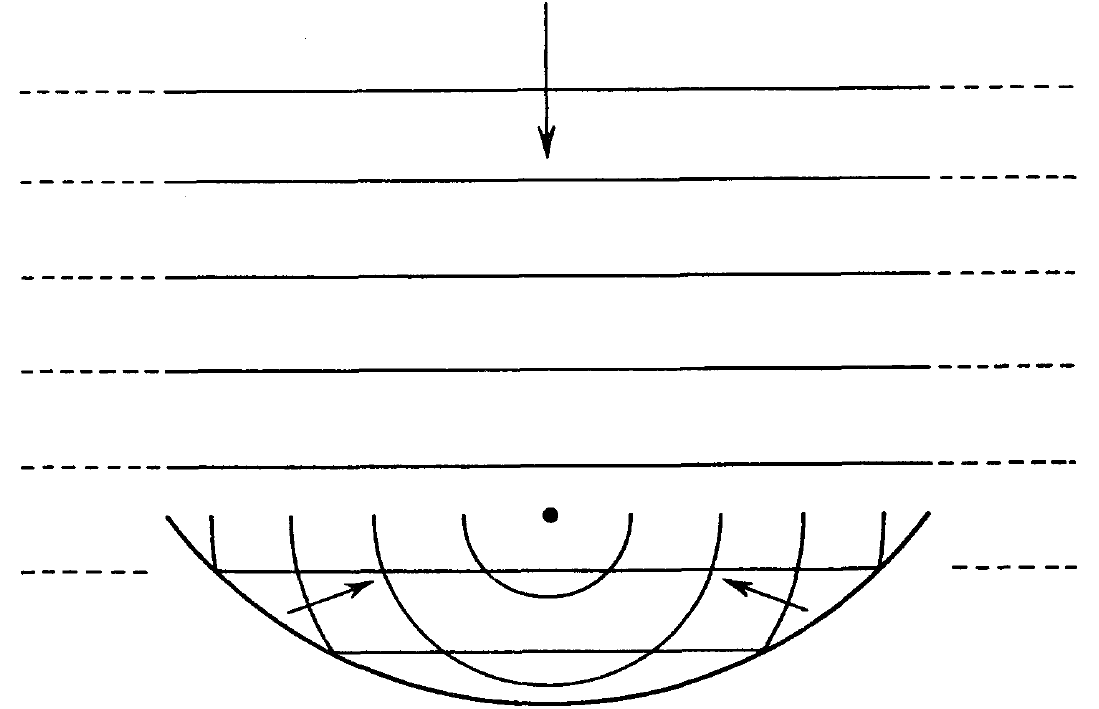
\includegraphics[width=0.4\textwidth]{images/diffraction_pattern.png}
  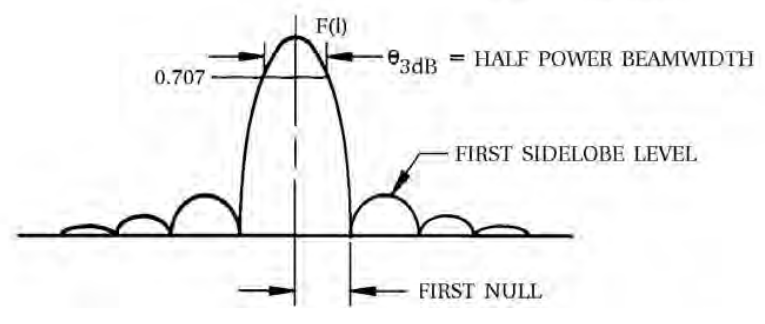
\includegraphics[width=0.5\textwidth]{images/radiation_pattern.png}
  \caption[Collection of electromagnetic wave energy and response]{Here the wave pattern of a parabolic aperture is 
  illustrated with a single cutting plane. The interference pattern created at the focus (illustrated on the right) is analogous to the interference pattern 
  of visible light when passing through a single narrow slit. Directional antennae form a discernible primary lobe, with several minor lobes of decreasing magnitudes to
  either side. The beam width of the primary lobe is usually defined as being at the level where the electric intensity is halved (around $1/\sqrt{2}$ of the maximum response).
  At approximately $\frac{\lambda}{D}$ the ``first null'' appears ($D$ is the diameter of the aperture). This is the first point of complete destructive interference. When synthesizing
  an image  of a source which extends beyond the primary beam, one will notice a severe drop in the intensity of its edges. Images taken from \textit{Radiotelescopes} \cite{christiansenradiotelescopes} 
  and \textit{Synthesis Imaging II} \cite{taylor1999synthesis} (left and right, respectively).}
  \label{diffraction_pattern}
 \end{mdframed}
\end{figure}

When placing the antenna back into a more realistic context: relatively close to the ground and taking the resistance of the feed connecting the antenna
to measuring equipment into account, this radiation pattern changes considerably to a so-called ``absolute'' beam pattern.
As expected the ground and any large nearby object will act as a reflector. Although the intensity of the reflection will vary depending
on how level the surrounding terrain is and its conductivity (dry or wet conditions) it cannot simply be ignored. Because the reflected wave may
be out of phase depending on the height of the antenna and its declination, portions of the primary beam in the vertical direction
may experience significant destructive interference.

The gain, $G$, of the antenna is defined as the ratio of radiation intensity collected in a given direction (as when emitted by a highly 
directional source), to the intensity that would have been obtained when receiving from an isotropic source. This definition includes feed losses
due to ordinary resistance and is obviously direction dependent. For our discussion on radio telescopes, however it is much more useful to think in terms of 
the effective area of the antenna. The effective area is defined in terms of the gain of the antenna as:
\begin{equation*}
 A_e = \frac{G\lambda^2}{4\pi}
\end{equation*}
Assuming absolutely no losses occur in the measured electric density and no phase errors are introduced, this effective area will approach the geometric area of telescope in the direction
of maximum constructive interference. In practical application this is never achieved. The effective collecting area of the telescope is limited by a variety of
factors including, but not limited to, aperture surface deformation, blockage of the collecting area by support struts and the radiating properties of the feed.

It is worth pointing out that these radiating patterns are measured in the far field of the antenna (at distances at least $\frac{2D^2}{\lambda}$ from
the antenna where $D$ is the diameter of the aperture) to avoid any near-field reactive effects. The gain of an antenna must therefore be seen as a 
far-field concept.

In addition to the effective collecting area just defined all antennae are only considered effective for a limited spectrum of frequencies (or ``bandwidth''). 
This may be either a narrow or a wide band of frequencies. Size is one of the factors governing effectiveness when it comes to bandwidth. 
Although there are no hard and fast rules about the size of antennae, a general rule of thumb is that antennae smaller than $0.5\lambda$ are considered electrically small and antennae more than 
about $100\lambda$ are considered electrically large, and are capable of attaining much higher gains in the case of directional antennae.

For astronomical purposes it is \textit{very important} to have an antenna much larger than $\lambda$ in order to increase both sensitivity 
and resolution. Although large objects may easily be resolved if they are smaller than the primary beam in the response pattern of the antenna, 
the resolution of finer details depends squarely on the angular resolution of the observing telescope:

\begin{equation*}
 \text{angular resolution} \propto \frac{\lambda}{D}
\end{equation*}
where $D$ is the aperture diameter.

Small telescopes will smear finer detail, and point sources right next to each other may not be discernible. The angular resolution is
an indication of the minimum distance at which two point sources can be separated and still be discernible. This sheds some light on astronomers'
neverending pursuit of larger and larger antennae, as evident by the Arecibo observatory in Puerto Rico (Figure \ref{fig_arecibo}).

\begin{figure}[ht]
 \begin{mdframed}
 \centering
 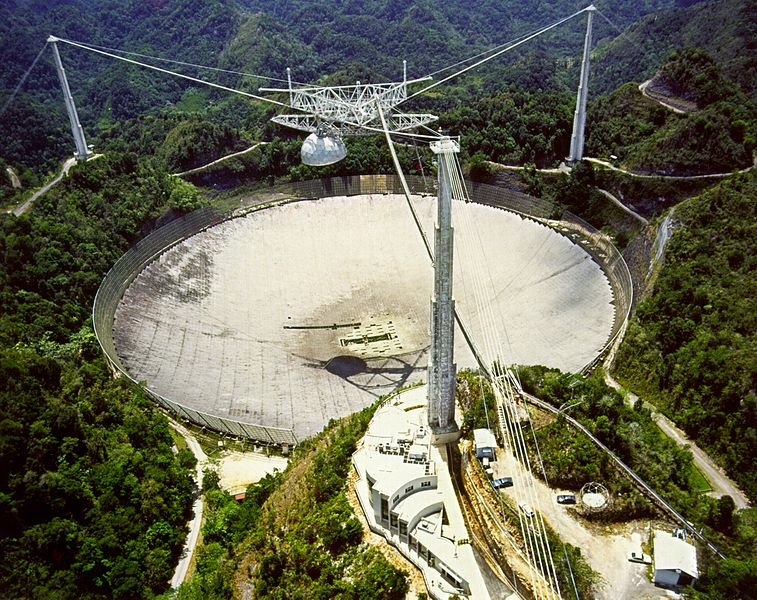
\includegraphics[width=0.7\textwidth]{images/arecibo.jpg}
 \caption[Arecibo Observatory]{At a massive 305m diameter, the telescope at the Arecibo Observatory is amongst the largest single-aperture telescopes in the world. 
 Image courtesy of the National Oceanic and Atmospheric Administration (public domain).}
  \label{fig_arecibo}
 \end{mdframed}
\end{figure}

\subsection{Measurement}
For the sake of discussion and to simplify the mathematics we introduce the following simplifying assumptions about radio emission:
\begin{enumerate}
 \item Most radio sources emit their radiation outward uniformly in all directions (they are \textit{isotropic}),
 \item Sources have roughly the same brightness over their entire area (they are said to be \textit{quasi-monochromatic}), 
 \item The emission from any two astronomical sources (or any two points on a single source) is incoherent: it certainly
 varies with frequency and to some extent with time.
 \item That the distances over which these waves travel are far enough to consider them planar by the time they reach the 
 observing telescope.
\end{enumerate}

The energy available at the output terminals of a single aperture antenna will be roughly proportional to the electrical intensity per unit area per unit frequency on the 
collected planar wavefront. This is the electrical flux density, $S$, measured in units $\text{W}\text{m}^{-2}\text{Hz}^{-1}$. It is useful to remind the reader that power is proportional to the square voltage and may 
practically be used interchangeably.

A single antenna telescope measures its power over a limited bandwidth and effective area $A_e$, as explained earlier. Assuming
no attenuation or delays are introduced by the atmosphere or equipment, and that the antenna measures two complementary polarizations, this 
means the total power measured by the telescope when pointed in the direction of a single point source is: 
\begin{equation*}
W = A_e.S.\Delta\nu
\end{equation*}

Using this total power relation it is easy to see the advantage of averaging several bands together to observe sources of \emph{continuum emission}, although
observation of spectral line emission (such as the absorption line of abundant neutral hydrogen at 21cm, along with other common elements) is also very 
important when tracking the evolution of the universe.

Before deriving a more formal mathematical framework to describe the measurements taken of sources on the celestial sphere it is necessary to introduce a 
rectangular coordinate system centered on the focus of the antenna, tilted such that w points in the direction of the maximum response, and u and v are the 
orthogonal horizontal and vertical cutting planes respectively. u, v and w are 
measured in wavelengths, and therefore measured in meters. The direction of a point on the sky (a unit sphere) is given by the 
direction cosines, measured according to the local frame. These cosines are denoted by l, m and n respectively (note that $l^2 + m^2 + n^2 = 1$). 
Both $l$ and $m$ may range between $\pm\pi \text{ radians}$.

Now let $\Omega$ be a \textit{small} solid angle subtended by a very small area. This solid angle is measured in square radians (steradians or ``sr''). A visualization 
of the measured flux density falling on an infinitesimal area of telescope is given in Figure~\ref{fig_measuring_source_brightness}. The flux density measured 
per steradian over the entire solid angle per unit frequency must then be 
  \begin{equation}
    p \approx \int_{\Omega}{A(l,m).I(l,m)\cos{\theta}d\Omega}
    \label{REF_EQN_SINGLE_ANTENNA}
  \end{equation}
where\\
  $p$ is traditionally measured in Janskies ($10^{-26}.W.m^{-2}.Hz^{-1}$)\\
  $I$ is the flux density measured per unit steradian: $I(l,m) := \frac{\Delta S(l,m)}{\Delta\Omega}$\\
\begin{figure}[ht]
\begin{mdframed}
 \centering
 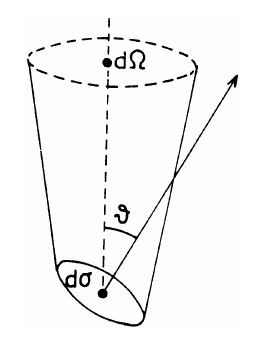
\includegraphics[width=0.2\textwidth]{images/measuring_source_brightness.png}
 \caption[Source brightness]{Flux density collected by a small area on the antenna. Image taken from \textit{Tools of radio astronomy}\cite{wilson2009tools}.}
 \label{fig_measuring_source_brightness}
\end{mdframed}
\end{figure}

In reality multiple sources will be contributing to this integral, each at a separate angle to the pointing center. The integral should therefore be taken over 
all contributing sources. It was assumed that these radiate independently of each other. Furthermore, the effects of the atmosphere, specifically frequency 
dependent delays and phase rotation, as well as tropospheric effects have been downplayed. The pointing accuracy and radiative properties of the antenna including its internal 
temperature, polarization leakage, were also downplayed. Some of these effects can be corrected for through direct calibration and model-fitting techniques, 
but the exact details are beyond the scope of this introductory discussion. Typically calibration can be broken up into three areas:
\begin{itemize}
 \item \textbf{Direct calibration} involves data flagging. This type of calibration is normally used to mark broad portions of the data that is known to be invalid, due to for example
 technical malfunction or terrestrial radio interference. Modern radio astronomy software, for example the CASA reduction suite, have tools for performing this type of calibration.
 \item \textbf{Calibration through known calibrator sources and a priori information} 
 \item \textbf{Self-calibration processes} are iterative processes which typically involve model fitting algorithms and techniques.
\end{itemize}

For more details the reader is referred to Synthesis Imaging II \cite[Lectures 3, 5, 8 and 10]{taylor1999synthesis}. In the measurement section of the next chapter
we will refer to a general model which may be used to describe both atmospheric and antenna terms and can be used for self-calibration processes.

\section{Aperture synthesis with array telescopes}
\subsection{Overview}
As pointed out in the previous section the angular resolution is constrained by the diameter of the telescope. For longer 
wavelengths very large directional antennae are needed to achieve good angular resolution. Unfortunately,
there are material constraints, increased maintenance costs and difficulties in steering associated with large telescopes. 
Luckily, it is not essential to build a filled aperture in order to create a reasonably efficient directional antenna. It is 
also possible to leave out large portions of the antenna aperture to create a directional antennae of significantly 
reduced weight (which is much cheaper to build). The obvious effect is a decrease in effective collecting area
and therefore decreased sensitivity.

Array telescopes can be thought of as a special case of these unfilled apertures. The very simplest way of creating such
a telescope will be to simply add the signals from all the receivers together before measurement, in order to form a 
basic ``total power'' telescope. This is only possible if the signals being added together are reasonably \textit{coherent}. If they
are significantly out of phase the signals will experience destructive interference and the telescope will be
rendered useless. For the sake of discussion, however, it is assumed that the distances between antennae are fully accounted for: the wavefront 
collected at different locations will simultaneously arrive at the measurement equipment shortly 
thereafter, and the increased impedance associated with longer transmission lines is duly considered.

Using an array it is possible to ``synthesize'' a single aperture telescope that encompasses the entire array. This
basic idea is known as \textit{aperture synthesis}. It does, however, pose a serious conundrum: only some areas will be well covered, whereas
large areas may not be covered at all. As we see later this produces smearing in the synthesized images and is a topic of much 
discussion by itself.

The resolving power obtained from such a synthesized aperture depends on the distance between the furthest separated 
telescopes, and can be expressed as:
\begin{equation*}
 \text{angular resolution} \propto \frac{\lambda}{B} \text{ if } D\ll B
\end{equation*}
where $D$ is the diameter of the largest aperture in the array and $B$ is the length of the longest \textit{baseline} 
(the vector defined between the positions of pairs of antennae: $\vec{b}_{pq}=P_p - P_q$). $\lambda$ is the observed wavelength.

Since Martin Ryle and his collaborators made their pioneering observations using array telescopes there has been
a significant drive towards building arrays of ever-increasing size. In applications where angular resolution is
the one of the dominant factors it is even possible to connect up telescopes located on different continents, or even orbiting satellites.
This is appropriately called \textit{Very Long Baseline Interferometry}. Avid readers may refer to the survey 
conducted by Middelberg et al. \cite{middelberg2008high} for a good introductory overview of VLBI. In the next section we discuss
what is meant by an interferometer and why array telescopes are referred to as radio interferometers

\subsection{Measurement}
It is also possible to think of arrays using a more physical model. These telescopes measure what is commonly referred 
to as the \textit{spacial coherence} of a source. A simple analogy for how array antennae work from a physical 
perspective would be to think of a point disturbance in a bowl of water. If the amplitude is measured by two calibrated 
sensors at the same location, the readings obtained should be exactly equal at any point in time. As the sensors are 
spaced further and further away from each other, but remain equidistant to the source, one would expect the readings to still
be the same - since the waves propagate outward at the same speed and with the same amplitude. The degree to which
the two measurements correspond at any point in time will tell the observer how coherently the waves are propagating outward.
If one of the sensors is moved slightly further away from the disturbance, the delay between the measurement taken by
the first and second sensors will tell the observer something about the position of the disturbance.

If this bowl of water analogy is scaled up to monstrous proportions, and the water is replaced with free space, it 
resembles an array telescope. Since the source is assumed to be sufficiently far away, each electromagnetic wave crest 
will be measured by two (or more) directional antennae at exactly the same time, provided those antennae point
towards the same sky position. Just as with the bowl of water analogy if the source is slightly offset from the pointing centre of the
telescope, the phase delay between the arrival of the wave front at two separate antennae will tell the observer something about its 
offset from the pointing centre. Refer to Figure~\ref{fig_interferometer} for an illustration.

\begin{figure}[ht]
 \begin{mdframed}
 \centering
\psscalebox{1.0 1.0} % Change this value to rescale the drawing.
{
\begin{pspicture}(0,-5.5175757)(8.341955,5.5175757)
\definecolor{colour0}{rgb}{0.003921569,0.003921569,0.003921569}
\definecolor{colour1}{rgb}{0.0,0.047058824,1.0}
\rput{-226.70288}(-1.2319194,-5.399251){\psarc[linecolor=black, linewidth=0.02, fillstyle=solid,fillcolor=colour0, dimen=outer](0.5495573,-2.9655557){0.6944444}{7.8650684}{7.975039}}
\rput{-225.20427}(1.9264939,-5.7953396){\psarc[linecolor=black, linewidth=0.02, fillstyle=solid,fillcolor=colour0, dimen=outer](2.1695573,-2.4966667){1.31}{85.28396}{184.43335}}
\rput{-225.20427}(10.743828,-9.466027){\psarc[linecolor=black, linewidth=0.02, fillstyle=solid,fillcolor=colour0, dimen=outer](7.3422847,-2.4966667){1.31}{85.28396}{184.43335}}
\psline[linecolor=black, linewidth=0.02, arrowsize=0.05291666666666667cm 2.0,arrowlength=1.4,arrowinset=0.0]{->}(3.0904665,-0.43575758)(2.1177392,-3.3266666)
\psline[linecolor=black, linewidth=0.02, arrowsize=0.05291666666666667cm 2.0,arrowlength=1.4,arrowinset=0.0]{->}(8.245012,-0.4630303)(7.2722845,-3.3539393)
\psline[linecolor=black, linewidth=0.02, linestyle=dashed, dash=0.17638889cm 0.10583334cm](7.2722845,-3.3266666)(2.5904665,-1.9539394)
\rput{-19.51438}(1.2411542,0.5933079){\psarc[linecolor=black, linewidth=0.02, dimen=outer](2.3457046,-3.3121789){0.36926407}{33.895622}{125.547806}}
\psline[linecolor=black, linewidth=0.02, arrowsize=0.05291666666666667cm 2.0,arrowlength=1.4,arrowinset=0.0]{<->}(2.6995573,-3.2171428)(6.766224,-3.2266667)
\rput[bl](2.5449786,-2.984176){$\alpha$}
\psline[linecolor=red, linewidth=0.02, arrowsize=0.05291666666666667cm 2.0,arrowlength=1.4,arrowinset=0.0]{->}(7.270986,-3.312381)(7.213843,-0.4409524)
\rput[bl](7.070986,-0.32666665){$\vec{s_0}$}
\psline[linecolor=colour1, linewidth=0.02, arrowsize=0.05291666666666667cm 2.0,arrowlength=1.4,arrowinset=0.0]{->}(7.7836843,-2.2901587)(8.083684,-1.5473015)
\rput[bl](8.018605,-2.0726984){$\vec{s}$}
\psarc[linecolor=black, linewidth=0.02, dimen=outer](7.377335,-2.5481944){0.16736111}{0.0}{131.89452}
\rput[bl](7.299557,-2.7266667){$\theta$}
\psline[linecolor=black, linewidth=0.02, arrowsize=0.05291666666666667cm 2.0,arrowlength=1.4,arrowinset=0.0]{<->}(2.4450119,-1.9175757)(2.0086482,-3.2872727)
\rput[bl](1.4995573,-2.5842423){$\vec{b}\cdot\vec{s}$}
\rput[bl](4.0086484,-3.7236364){$||\vec{b}|| = L$}
\rput[bl](0.16622397,-2.3903031){$\tau=\frac{\vec{b}\cdot\vec{s}}{c}$}
\psline[linecolor=black, linewidth=0.02](2.1177392,-3.8084848)(2.0934968,-4.9721212)(4.493497,-4.9842424)
\psline[linecolor=black, linewidth=0.02](4.8934965,-4.9842424)(7.2934966,-4.9842424)(7.2934966,-3.7963636)
\psframe[linecolor=black, linewidth=0.02, fillstyle=solid,fillcolor=colour0, dimen=outer](4.917739,-4.7296968)(4.4813757,-5.2145452)
\rput[bl](3.9601634,-5.5175757){correlator}
\end{pspicture}
}
  \caption[Array-base observation]{In this simplified illustration of a two antenna array the incoming wavefront being measured is produced
  by a single source in the direction of $\vec{s}$, offset at an angle $\theta$ from the pointing center,$\vec{s_0}$, of the telescope.
  Here, it is assumed that the pointing center is also the center of maximum response and where the delay between incoming signals
  is exactly zero. The \textit{correlator} measures the degree to which the signals measured at the two antennae correspond 
  (both in phase and amplitude), by measuring the degree of spacial coherence of the incoming wavefront. For now we can assume
  the entire radio interferometer is on level ground, and importantly that the measured wavefronts are planar. As already mentioned
  the time delay, $\tau$ between the arrival of the wave front between the two antennae corresponds to a phase delay in the measured
  signal. $c$ is the speed of light.}
  \label{fig_interferometer}
 \end{mdframed}
\end{figure}

These differences in phase, which depend on the angle of the incoming wavefront with respect to the pointing center, will 
produce an interference phase pattern that is analogous to Young's double slit experiment, where an interference pattern 
is formed on a screen when light passes through two small slits (separated by a distance $L$) somewhere in front of the 
screen. Here the size of the slits are small in comparison to both $\lambda$ and $L$. The first null point occurs at a distance 
proportional to $\frac{\lambda}{L}$. The only major difference between the two contexts is that the antennae should be
viewed as narrow slits. Waves from directions $\theta=n\pi, n\in\mathbb{Z}$ will undergo constructive interference, but 
those from directions $\theta = (n + \frac{1}{2})\pi$ will be invisible to the interferometer. Such an interference 
pattern is not ideal when resolving large structures.

One way around this problem is to take an additional delayed measurement 
at $\tau_{delay}=\frac{\pi}{2}$ radians and combine this ``sine interference pattern'' with the original 
``cosine interference pattern''. In theory this improves the signal to noise ratio by a factor of roughly $\sqrt{2}$ and will 
produce a response pattern that is sensitive over a wider range of angles. From this point forward whenever referring to the 
correlator we will be considering the \textit{complex} correlator. It is convenient to think of the measurements made by such a complex 
correlator in terms of the polar form of complex numbers. Recall Euler's identity:
\begin{equation*}
 e^{i\theta} = \cos{\theta} + i\sin{\theta}
\end{equation*}

As the reader may suspect the mathematical treatment of the measurements taken by these array telescopes are analogous
to that of a single aperture telescope, except that in the single antenna case the telescope measures the cosine modulated
flux density directly. Here instead the signals are combined and measured by the external correlator. The mathematical 
discussion is very similar to that of a single antenna telescope, but will be that of a complex measurement, 
instead of only dealing with the real domain.

Up to this point it has been assumed that the signal will not vary over time, and that the measurement equipment is perfect; it 
does not delay or attenuate the collected signal (commonly referred to as the \textit{instrumental gain}). In reality, however, 
such perfection is never attained. The sensitivity of the complex interferometer depends firmly on the total collecting area 
as we already discussed, the resistivity (and associated temperature) of the equipment, including the antenna and amplifying 
electronics, the bandwidth being integrated as mentioned previously and the integration time. We state without proof here 
that:

\begin{equation}
 \sigma_{noise} \propto \frac{T_{sys}}{\sqrt{\Delta\nu\Delta\tau_{integration}}}
\end{equation}

At a physical level, sources do vary slightly over time, although we expect their average intensity to be centered around 
some mean. The instrumentation used for measuring will also contribute some variation in noise level that have to 
be corrected for on a regular basis. With this in mind it is important to make yet another assumption about 
the physical processes being measured: sources \textit{do not} vary significantly from their mean intensity 
on a day to day basis. The obvious exception to this are the fast transient sources like pulsars. 
These sources must be observed over very short periods of time, and by implication must be relatively bright.
Fainter sources have to be observed for much longer to be discernible from noise. This brings up the problem
of tracking stellar sources.

For this discussion refer to Figure~\ref{fig_celestrial_coords} for a visual reference. Due to the rotation 
axis of the earth sources on the celestial sphere will appear to move both in azimuth and elevation, moving from East to West.
However, it may not be immediately apparent that the rising and setting positions of a source (for example the sun) with respect to the local horizon
do not remain fixed throughout the duration of a year. If one were to point a camera due East to monitor the sunrise
over the course of one year, the rising position will appear to oscillate around true East over the course of the year. Only at two 
points during the year will the sun rise due East - these are known as the spring and autumn equinoxes. At these points the 
plane containing the earth's equator intersects the sun. This is the reason why the sun will appear to move along different star 
constellations throughout the year. Hence astronomers need a coordinate system that measures the earth's rotation with respect 
to the stars and not the sun in order to accurately fix the position of sources for long term observation (on the scale of decades).

In order to track sources over a prolonged period of time it is also very useful to convert their coordinates to a reference 
frame where the path of a source is determined only by an hour angle. In this reference frame the equator of the earth
is projected out onto the unit celestial sphere mentioned previously. The declination of a source is the distance
along the great circle connecting the North Celestial Pole (NCP, the projection of the magnetic north pole onto the unit sphere)
and the projected equator.

\begin{figure}[h]
 \begin{mdframed}
 \centering
 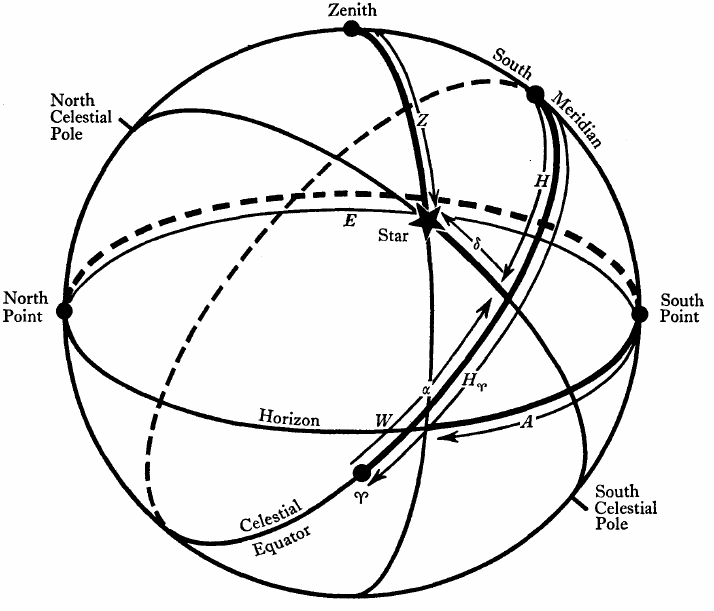
\includegraphics[width=0.75\textwidth]{images/equatorial_coords.png}
 \caption[Equatorial coordinate system vs the local horizon]{The angular coordinates of a point in the sky can be measured in terms of declination ($\delta$) and either right-ascension ($\alpha$ or R.A.) or the local sidereal time (hour angle) at the position where
 observations are taken. The first point of Aries (\Aries) is the position of sunrise at the March Equinox. The celestial equator is simply Earth's equator projected onto the celestial sphere. There is normally a slow precession in the Earth's
 axis and this has to be corrected for, based on some reference point in time (an epoch). The last epoch at the time of writing was at noon January 1, 2000. Zenith here refers to the point exactly above the observer's head. See Radiotelescopes 
 \cite[Appendix 4]{christiansenradiotelescopes} for more information.}
  \label{fig_celestrial_coords}
 \end{mdframed}
\end{figure}

Next we need to amend the local coordinate system defined previously for a single antenna telescope to be relative to some fixed location in order to derive a mathematical model for an interferometer. 
All the antennae in an array will be measured relative to this new coordinate frame. We assume a single antenna is picked as the reference point and all the other antennae 
positions are measured relative to this ``reference antenna''. 

This local Euclidian frame has the regular components X, Y, Z. If we use a right-handed system where X points in the direction 
of the $0^h$ hour hand, at a declination of $0^{\circ}$, Y lies on the same plane as X, but points to $18^h$ and Z points straight up 
towards the North Celestial Pole (NCP), then the baseline is given by the following relation, where $H_0$ and $\delta_0$ are the 
respective hour angle and declination of the phase reference center and $\lambda$ is the wavelength corresponding to the center 
frequency of the receiver. Here u, v, w are given by:
\begin{equation}
 \label{EQN_RIGHTHANDED_SYSTEM}
 \left[\begin{array}{c}
     u\\
     v \\
     w \\
    \end{array}\right] = \frac{1}{\lambda}
 \left[\begin{array}{c c c}
     \sin{H_0} 			& \cos{H_0}			& 0 \\
     -\sin{\delta_0}\cos{H_0} 	& \sin{\delta_0}\sin{H_0}	& \cos{\delta_0}\\
     \cos{\delta_0}\cos{H_0} 	& -\cos{\delta_0}\sin{H_0}	& \sin{\delta_0}\\
    \end{array}\right]   
 \left[\begin{array}{c}
     L_X \\
     L_Y \\
     L_Z \\
    \end{array}\right]
\end{equation}
The direction cosines towards a point on the celestial sphere are still given in relation to this relative u, v, w coordinate frame.
A similar left-handed convention can just as easily be defined ($\alpha_0$ is the right ascension of the pointing center):
\begin{equation}
 \left[\begin{array}{c}
     u\\
     v \\
     w \\
    \end{array}\right] = \frac{1}{\lambda}
 \left[\begin{array}{c c c}
     -\sin{\alpha_0} 			& \cos{\alpha_0}		& 0 \\
     -\sin{\delta_0}\cos{\alpha_0} 	& -\sin{\delta_0}\sin{\alpha_0}	& \cos{\delta_0}\\
     \cos{\delta_0}\cos{\alpha_0} 	& \cos{\delta_0}\sin{\alpha_0}	& \sin{\delta_0}\\
    \end{array}\right]   
 \left[\begin{array}{c}
     L_X \\
     L_Y \\
     L_Z \\
    \end{array}\right]
\end{equation}

Ignoring the effects of polarization, the directional antenna gain (the beam, as before) and any atmospheric effects
for the moment, the correlator will measure values proportional to:
\begin{equation*}
    p(u,v,w) \approx \int_{sources}\int_{sources}{\left<E_p(\vec{s})E_q^*(\vec{s'})\right>e^{2\pi i\vec{p}\cdot\vec{s}}e^{-2\pi i\vec{q}\cdot\vec{s'}}d\Omega_pd\Omega_q}     
\end{equation*}

Here E is the flux density over a small area (stemming directly from equation~\ref{REF_EQN_SINGLE_ANTENNA}). The assumption that two sources at differing locations are 
not strongly correlated (in other words spatially coherent) and that the sources are very far away is essential in order to simplify this relationship between flux densities 
and correlator output. Still assuming both source direction vectors ($\vec{s}$ and $\vec{s'}$ from antennas $p$ and $q$ respectively) are unit vectors pointing to positions 
on the unit celestial sphere, this assumption implies that $<S_p(\vec{s})S_q^*(\vec{s'})> \neq 0$ only when $\vec{s} = \vec{s'}$. Also note that, since complex fluxes 
are being measured by the correlator, it is necessary to take the short time averages of the complex conjugate (denoted $^{*}$)
of one of the antennae in order to measure the total flux contributed by both components - otherwise the difference between
them will be measured! 
\begin{equation*}
  \begin{split}
    p(u,v,w) &\approx \int_{sources}{\left<E_p(\vec{s})E_q^*(\vec{s})\right>e^{-2\pi i(\vec{q} - \vec{p})\cdot\vec{s}}d\Omega}\\
    p(u,v,w) &\approx \int_{sources}{B(\vec{s})e^{-2\pi i(\vec{b}\cdot(\vec{s}))}d\Omega}\\
  \end{split}
\end{equation*}

Notice that the expression for $p$ is relative and depends only on the direction of each contributing source. Of course this
is all relative to the pointing centre of the telescope. We may multiply through by a complex exponential to add the appropriate 
delay, which ensures measurements are taken relative to the pointing center. It may help to think of this as measuring the
incoming (complex) flux from direction $\theta$ as shown in Figure~\ref{fig_interferometer}:
\begin{equation}
 \label{EQN_ONE_CORR_RIME}
 \begin{split}
 p(u,v,w) &\approx \int_{sources}{B(\vec{s})e^{-2\pi i(\vec{b}\cdot(\vec{s}-\vec{s_0}))}d\Omega}\\
	  &\approx \int\int_{sources}{B(l,m,n)e^{-2\pi i(ul+vm+w(\sqrt{1-l^2-m^2}-1))}\frac{dldm}{\sqrt{1-l^2-m^2}}}\\
 \end{split}
\end{equation}

By no means should this model be taken as a rigorous derivation, but we will use it nonetheless (and slightly amend it 
along the way). A more rigorous derivation is given by Romney in \cite{taylor1999synthesis}[ch. 4].

In reality averaging the flux over a small band of frequencies and, additionally, over short periods of 
time will result in smeared measurements. It is important to emphasize that the baselines between pairs of antennae are 
\textit{always} measured in terms of wavelength (and by relation frequency) as evident from Equation~\ref{EQN_RIGHTHANDED_SYSTEM}.
If one were to integrate over such limited bandwidth a problem becomes apparent: the correlator response
is modulated by $\Delta\nu\sinc{\pi\Delta\nu\tau}$ (sinc is defined as $\sinc{x} = \frac{\sin{x}}{x}$). As apparent from
Figure~\ref{fig_interferometer}, $\tau$ depends on the orientation of the baseline with respect to a source, as well as the length of the 
baseline. The correlator response will be maximum only when the source vector is normal to the baseline. Therefore the 
correlator must compensate for this delay, as well as continuously shift the fringe modulation function to the phase centre of the 
observed field.

Up to this point we have for simplicity only discussed correlator output between single feed antennae.
Just as in the case of a single antenna telescope, the response from such a correlator will only be sensitive to highly 
directional sources. The correlator may therefore additionally correlate all four combinations between the two orthogonal 
feeds of each antenna to form a 2x2 matrix of short time averages. Without any loss of generality the flux density 
average ($B$) in equation~\ref{EQN_ONE_CORR_RIME} can be replaced by four averages. The exponential term 
then becomes a scalar 2x2 matrix.

The four Stokes parameters are an easy way to describe the polarization of the measured electromagnetic field. These 
are non-physical quantities, but they conveniently express the degree to which the field is linearly or circularly polarized
(and anything in between). Each of the parameters (Q, U and V) are linearly independent and describe a position on the 
Poincar\'e Sphere (figure \ref{fig_poincare}). I is the total measured intensity. The coordinates of Q, U and V are
those given by:
\begin{equation}
\begin{split}
Q &= I\cos{2\chi}\cos{2\psi}\\
U &= I\cos{2\chi}\sin{2\psi}\\
V &= I\sin{2\chi}\\
\end{split}
\end{equation}

\begin{figure}
\begin{mdframed}
\centering
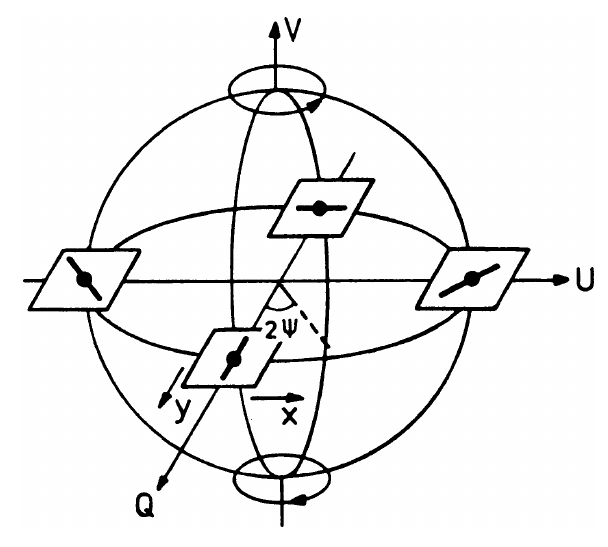
\includegraphics[width=0.45\textwidth]{images/poincare_sphere.png}
\caption[The Poincar\'e Sphere]{The Poincar\'e Sphere gives a visualization of the different polarizations in an electromagnetic field. The angles $2\psi$ and
$2\chi$ are the angles in a polar coordinate system, with each point on the sphere corresponding to a unique polarization. At $2\chi=0$ (the equator) the polarizations
are either linear (Q) or orthogonal (U). The northern latitudes ($2\chi > 0$) contain right-handed circular polarization, while the southern hemisphere
contains the left-handed circular polarizations. $I$ is not linearly independent and describes the total flux of the electromagnetic wave: 
$I = E_1^2 + E_2^2$ \cite{wilson2009tools}}
\label{fig_poincare}
\end{mdframed}
\end{figure}

In instances where all of these components are available the observer will be able to compute the polarization of
the observed radiation. If the feeds of both antennae are orthogonal circular feeds the relation to
the the four Stokes parameters is given by
\begin{equation}
    \left[\begin{array}{c c}
     <e_{R_p}e_{R_q}^*> & <e_{R_p}e_{L_q}^*> \\
     <e_{L_p}e_{R_q}^*> & <e_{L_p}e_{L_q}^*> \\
    \end{array}\right] \approx 
    \left[\begin{array}{c c}
     I + V & Q + iU \\
     Q - iU & I - V \\
    \end{array}\right] = B
\end{equation}

For linear orthogonal feeds the relationship is slightly different \cite{2011A&A...527A.106S}:
\begin{equation}
    \left[\begin{array}{c c}
     <e_{X_p}e_{X_q}^*> & <e_{X_p}e_{Y_q}^*> \\
     <e_{Y_p}e_{X_q}^*> & <e_{Y_p}e_{Y_q}^*> \\
    \end{array}\right] \approx 
    \left[\begin{array}{c c}
     I + Q & U + iV \\
     U - iV & I - Q \\
    \end{array}\right] = B
\end{equation}

Equation~\ref{EQN_ONE_CORR_RIME} may thus be rewritten to take multiple polarizations, equipment gains and directional effects into account through a \textit{Jones} matrix
formulation, presented by Oleg Smirnov in a series of papers where he discusses their implications for telescope calibration \cite{2011A&A...527A.106S,2011A&A...527A.107S,2011A&A...527A.108S,2011A&A...531A.159S}:

\begin{equation}
\label{eqn_RIME}
    V_{pq} = G_p(t,\upsilon)\left(\int\int_{sources}D_p(l,m,t,\upsilon)BK_{pq}D_q(l,m,t,\upsilon)^H\frac{dldm}{\sqrt{1-l^2-m^2}}\right)G_q(t,\upsilon)^H
\end{equation}
where $K = e^{-2\pi i(u_{pq}l+v_{pq}m+w_{pq}(n-1))}
    \left[\begin{array}{c c}
     1 & 0 \\
     0 & 1 \\
    \end{array}\right]$ and the G terms are the direction-independent effects, while the D terms are dependent on the direction of 
    the source in l,m space. $J^H:=J^{*^T}$ indicates the Hermitian transpose (the transpose of the complex conjugate matrix of J)\\
    
We shall henceforth refer to this relation as the \textit{Radio Interferometric Measurement Equation (RIME)}. 
The fundamental assumption here is that all effects on the measured intensities are linear and can therefore be 
written as two-dimensional matrices. Each antenna will then have its own set of corrections. They 
include corrections for Faraday rotation, ionospheric effects, tropospheric effects, the primary beam (and any rotation during
observation) and pointing error due to weather (wind for instance). These corrections only account for amplitude scaling and 
phase shifts and can be combined in a layered approach by multiplying several of these Jones terms together (note that the terms 
may not necessarily commute, so the order of multiplication is important). We will come back to exactly how these terms are applied
when discussing on how the RIME can be inverted.

Up to this point the formulation only accounts for two-element arrays. However, the linearity of the system allows us
to simply add multiple of these short term averages together. When discussing signal processing aspects more formally
it will become clear why this is possible. In practice, we can correlate the signal between all possible pairs of 
antennae and only reduce afterwards. This means that the data rates produced in correlation grows quadratically with 
number of antennae (ie., the number of possible baselines). This includes the auto-correlated baselines (correlation 
of each antenna with itself).
\begin{equation}
  \text{number of baselines } = \frac{n(n-1)}{2} + n
\end{equation}

Even if many baselines are used to synthesize an aperture it will still be
very sparsely sampled, especially when considering very large arrays. In fact, only a handful of small points will be 
sampled during a single integration period - hardly enough to represent a large continuous area! This means that 
the array telescope will be quite insensitive to very faint sources.

The solution to this problem lies in the beauty of the underpinning model just developed: the flux measurements
are \textit{relative}. Recall also the assumption that the intensity of the sources of electromagnetic radiation 
\textit{do not vary on a day-to-day basis}. This means an astronomer may fix one end of the baseline, and move the other
end. Some of the early radio telescope arrays did just this. Although many of the antennae were stationary a handful
of antennae were placed on tracks. These antennae would be moved to different positions to take multiple observations
of the sky.

Another, more promising, way of achieving this with much larger arrays is to use the rotation of the earth to rotate
the baselines radially with respect to the rotation axis of the planet. This may sound strange, but it 
follows naturally from the way the local coordinate frame was defined in Equation~\ref{EQN_RIGHTHANDED_SYSTEM}. If the
array tracks some point on the sky at some fixed declination over an extended period of time, the change in the hour
angle will rotate every baseline. This becomes more explicit once the equation is recast from parametric to implicit form. 

We start by obtaining the individual expressions for u,v,w in equation~\ref{EQN_RIGHTHANDED_SYSTEM}. If the expressions
for u and v are manipulated into the familiar form of an ellipse it is easy to show that the following
relation holds:
\begin{equation*}
 u^2 + \left(\frac{v-(L_Z/\lambda)\cos{\delta_0}}{\sin{\delta_0}}\right)^2 = \frac{L_X^2 + L_Y^2}{\lambda^2}
\end{equation*}

This ellipse is shifted along the v axis by $\frac{L_Z\cos{\delta_0}}{\lambda}$. The major axis has a length of 
$\frac{2\sqrt{L_X^2 + L_Y^2}}{\lambda}$. It also follows that at low declinations the baselines 
of a pure east-to-west array will be nearly parallel to the pointing direction of the telsecope.
Not only will the foremost antenna shadow the antennae behind it, but there will be little coverage of the u, v
frame and a very weak response if the $\tau$ is not corrected for. One way of improving u,v coverage is to add baselines
that are sufficiently perpendicular to the rotation of the Earth (as is done in the VLA). However, these baselines are rotated into
the w-direction and present a serious problem in imaging. We will come back to this when discussing wide-field imaging.

To make this more concrete consider a fictitious observation with the Extended Very Large Array. The antenna 
positions for all 27 antennae, available baselines and projected tracks are shown in Figure~\ref{fig_evla_observation}. With
increasing frequency these tracks expand outward. This means that it is possible to effectively increase coverage
by observing multiple frequencies and averaging them together. However, this will cause some radial smearing when
images are synthesized.

\begin{figure}[h]
 \begin{mdframed}
 \centering
 \begin{subfigure}[b]{0.3\textwidth}
  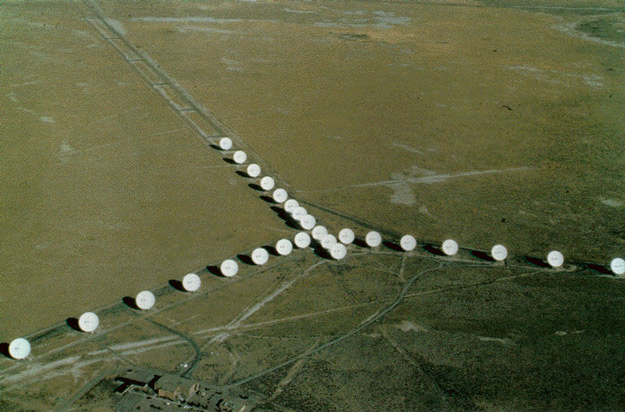
\includegraphics[width=\textwidth]{images/vla.jpg}
  \caption{}
 \end{subfigure}
 \begin{subfigure}[b]{0.3\textwidth}
  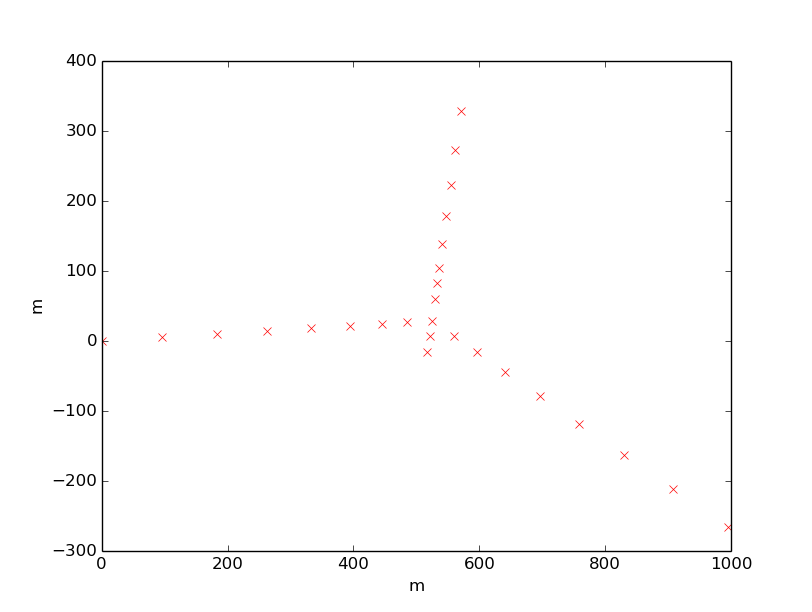
\includegraphics[width=\textwidth]{images/evla_observation/array_config.png}
  \caption{}
 \end{subfigure}
 \begin{subfigure}[b]{0.3\textwidth}
  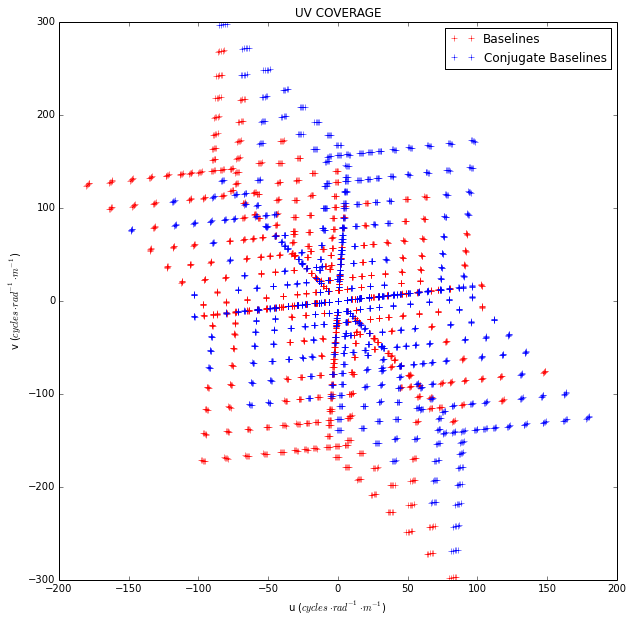
\includegraphics[width=\textwidth]{images/evla_observation/5min_snapshot_ncp.png}
  \caption{}
 \end{subfigure}
 \begin{subfigure}[b]{0.3\textwidth}
  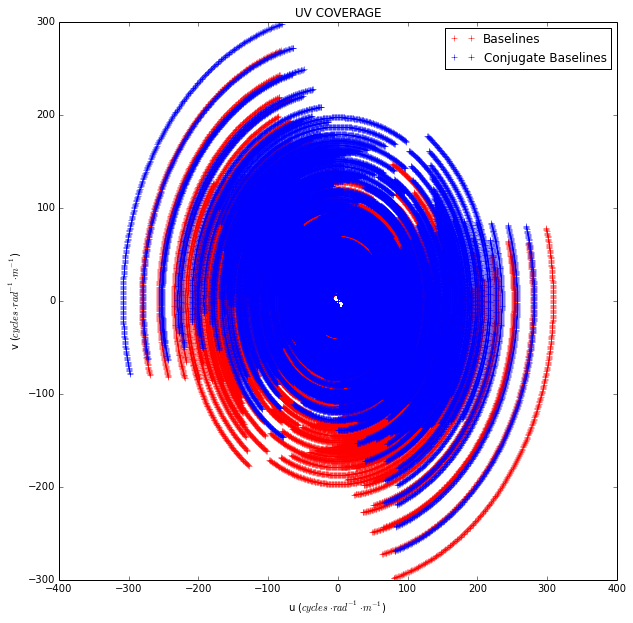
\includegraphics[width=\textwidth]{images/evla_observation/6hr_ncp.png}
  \caption{}
 \end{subfigure}
 \begin{subfigure}[b]{0.3\textwidth}
  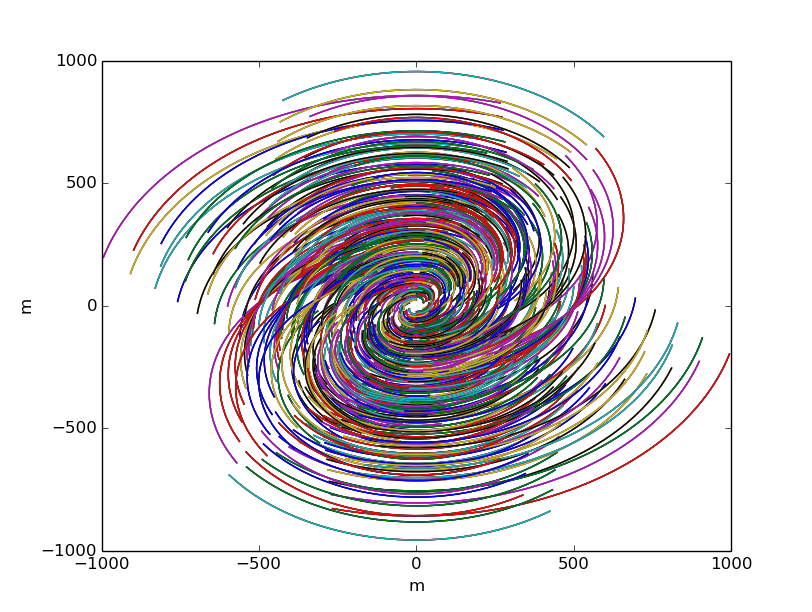
\includegraphics[width=\textwidth]{images/evla_observation/6hr_dec60.png}
  \caption{}
 \end{subfigure}
 \begin{subfigure}[b]{0.3\textwidth}
  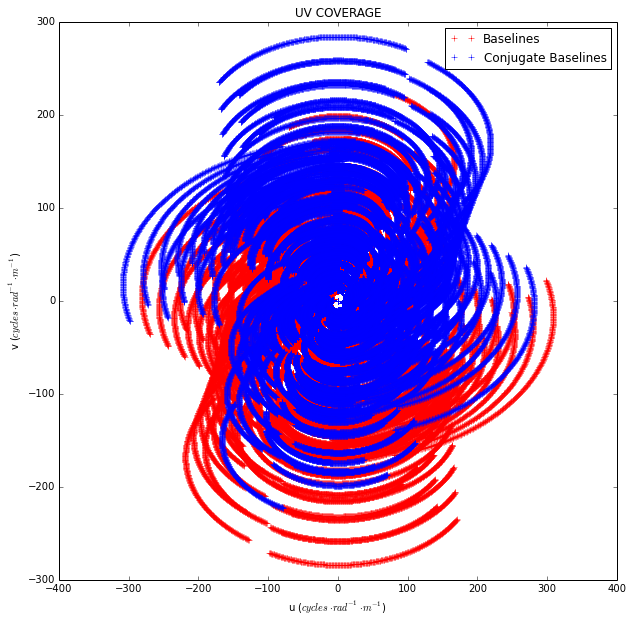
\includegraphics[width=\textwidth]{images/evla_observation/6hr_dec30.png}
  \caption{}
 \end{subfigure}
 \begin{subfigure}[b]{0.3\textwidth}
  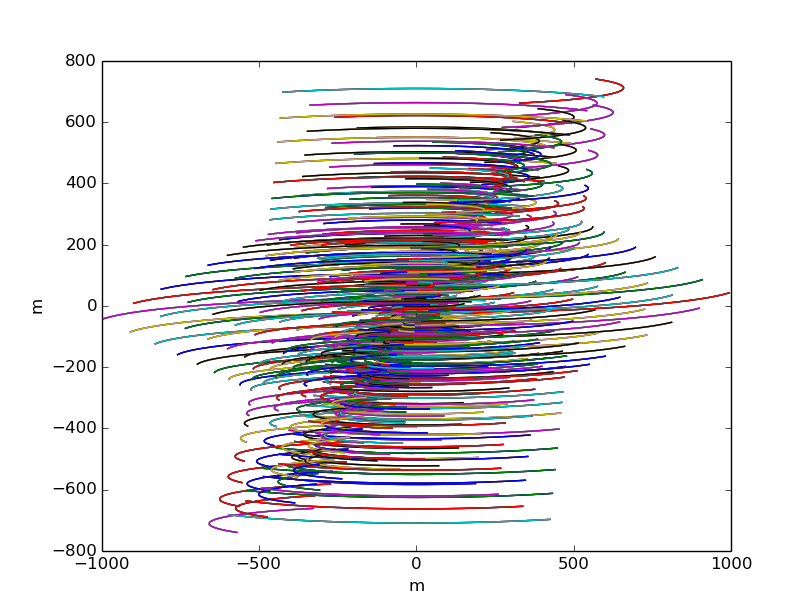
\includegraphics[width=\textwidth]{images/evla_observation/6hr_dec5.png}
  \caption{}
 \end{subfigure}
 \begin{subfigure}[b]{0.3\textwidth}
  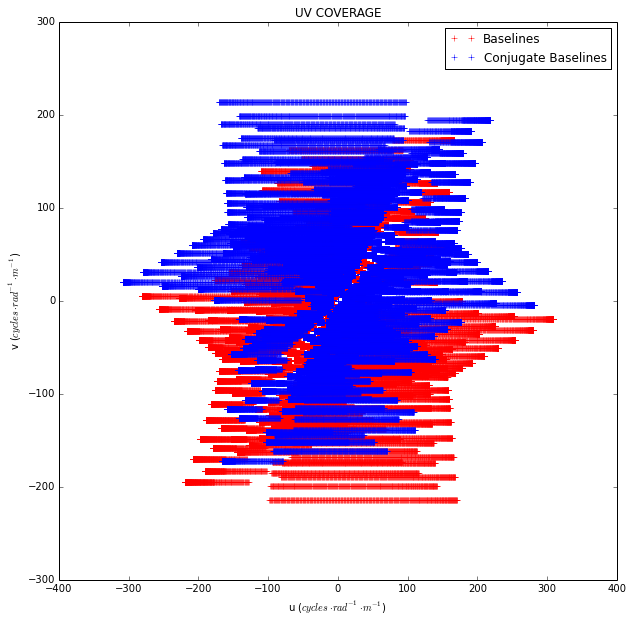
\includegraphics[width=\textwidth]{images/evla_observation/6hr_dec0.png}
  \caption{}
 \end{subfigure}
 \caption[u,v coverage]{Here the eliptical tracks from all baselines of the 27 antennae of the reconfigurable 
  Extended Very Large Array (National Radio Astronomy Observatory [New Mexico, US]) are shown at different declinations.
  In (a) a picture of the EVLA taken from \url{http://images.spaceref.com/news/2012/vla-625x412.jpg}. (b) shows the positions of the
  antennae when the array is in its compact ``D'' configuration. In (c) a 
  short (``snapshot'') 5min observation at NCP. In (d) a 6 hour observation at NCP. Figures (e)-(h) show 6 hour 
  observations for $\delta_0$ = $60^{\circ}$, $30^{\circ}$, $5^{\circ}$ and $0^{\circ}$ respectively.}
  \label{fig_evla_observation}
 \end{mdframed}
\end{figure}      
